\chapter{Software}
\label{software}
Følgende afsnit handler om softwarens opbygning. Afsnittet tager udgangspunkt i de specifikke funktionalitetskrav som står beskrevet i \autoref{Krav_til_funktionalitet}. På baggrund af kravenenes prioritering beskriver først hvordan et system overordnet kan se ud. Dernæst følger en  forklaring af hvordan programkoden virker.
 
\section{Overordnet system}
Funktionen, Afspil lyd, prioriteres som den vigtigste funktion hvorfor den implementeres først. Funktionen aktiveres som resultat af at brugeren interagere med en sensor.   
Programmet baseres på Arduino (https://www.arduino.cc) og Processing (https://processing.org). Kommunikation mellem Arduino og Processing foregår med USB kabel via protokollen Firmata (http://firmata.org/wiki/Download). 
 Arduinoen bruges til at aflæse sensornes analoge spændinger. De målte værdier sendes, via Firmata, videre til Processing som derefter bearbejder informationen.
 Ved at benytte Processing kan PC'ens egen hardware bruges til at bearbejde, lagre og afspille lydfilerne. Denne opsætning er valgt for hurtigt og let at konstruerer en fungerende prototype.  

\section{Programkode}
Programkoden udvikles i en iterativ proces. Følgende giver en forklaring af programkodens indhold og funktion.  

Til Arduinoen overføres protokollen Firmata som StandardFirmata. Derved kan funktionaliteten på arduinoen tilgås ved hjælp af Processing. For at  kontakt mellem Arduino og Processing er etableret, er det nødvendigt også at opsætte Processing til kommunikationen. Dette gøres ved at følgende eksekveres:

\begin{figure}[H]
\includegraphics[scale=0.8]{Figure/programkode01.png}
\end{figure}
  
Først importeres bibliotekerne: cc.arduino og processing.serial.
Derefter erklæres objektet Arduino som arduino. 
Til sidst initialiseres objektet i funktionen setup(). Her vælges fra Arduino.list() hvilket port arduinoen er tilsluttet. 

Næste skridt er at kunne afspille lydfiler i processing. Det gøres ved at følgende eksekveres:

\begin{figure}[H]
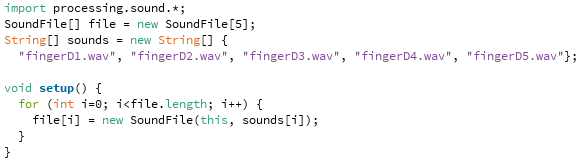
\includegraphics[scale=0.8]{Figure/programkode02.png}
\end{figure}  
 
Først importeres biblioteken: processing.sound.
Derefter erklæres et array af objektet Soundfile som file, med fem pladser.
Herefter erklæres et array af klassen Strings som efterfølgende initialiseres med navnene på de lydfiler der skal afspilles i programmet.
Til sidst initialiseres arrayet file, så hver plads i arrayet pares med en lydfil. Dette sker i funktionen setup via et for loop. Loopet fortsætter så længe der er pladser i arrayet file. 

   
Programmet kan nu kommunikere med arduinoen og de nødvendige lydfiler er klar til afspilning. Derudover skal der bruges tre variabler til at gemme vitale informationer. 

\begin{figure}[H]
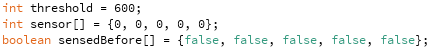
\includegraphics[scale=0.8]{Figure/programkode03.png}
\end{figure}  

En integer, threshold, gemmer grænseværdien for hvornår en aflæst sensorværdi er høj nok til at en lyd skal afspilles. 
Et integer array, sensor, sættes som udgangspunkt til nul og bruges efterfølgende til at gemme hver sensors aflæste værdi. 
Et boolean array, sensedBefore, sættes som udgangspunkt til false og bruges efterfølgende til at tjekke om en sensorværdi ellerede har overskredet grænseværdien og afspillet en lyd. 
 
Følgende beskriver forløbet som foregår ved funktionskaldet draw(). Umiddelbart er formålet med koden at afspille en lydfil hvis en aflæst sensorværdi overskrider threshold. Derudover sørger koden for at lydfilen kun afspilles en enkelt gang så længe sensorværdien er over threshold. 

\begin{figure}[H]
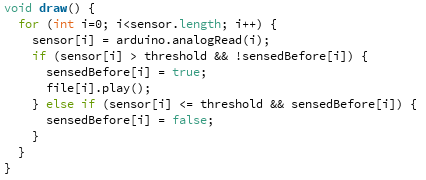
\includegraphics[scale=0.8]{Figure/programkode04.png}
\end{figure}  

Funktionen draw() er en indbygget funktion i processing som køres 60 gange i sekundet. 
Hver gang funktionen kaldes, igangsættes et for loop. For loopet er dimensioneret til at køres igennem en enkelt gang for hver plads i arrayet sensor. i, som starter på nul ved første gennemgang af for loopet, har en tilvækst på én ved hver gennemgang. i brugeres efterfølgende som en guide til hvor mange gange for loopet er kørt igennem. 
Det første der sker i for loopet er at en analog kanal på arduinoen aflæses, og værdien gennes i arrayet sensor. Den analoge kanal vælges ud fra i som til at starte med er 0. Derved aflæses kanal A0, analogRead(0), og gemmes på første plads i arrayet sensor, sensor[0], ved første gennemgang af for loopet. 
Det næste der sker er at den aflæste sensorværdi sammenlignes med threshold i et if statement. Hvis den aflæste sensorværdi er højere end threshold og booleanen, sensedBefore[0], er false, eksikveres koden inden i if statmentet. Er det tilfældet sættes sensedBefore[0] til true og lydfilen, file[0], afspilles.
Er det ikke tilfældet, fordi den aflæste sensorværdi ikke er over threshold eller fordi sensedBefore ikke er false, sammenlignes den aflæste sensorværdi igen med threshold i et else if statement. Denne gang for at tjekke om værdien er lig eller lavere end threshold. Hvis den aflæste sensorværdi er lavere end threshold og booleanen, sensedBefore[0], er true, eksikveres koden inden i else if statementet. Er det tilfældet sættes sensedBefore[0] til false.

For loopet gentages for hver plads i arrayet sensor. Ved hver gentagelse har i en tilvækst på én. Anden gang for loopet køres igennem er det derfor sensor[1] som er lig med værdien som aflæses på kanal A1, analogRead(1). Værdien sammenlignes med samme threshold, men nu er det booleanen sensedBefore[1] som skal være false for koden i if statmentet eksikveres. 

Figur \ref{fig:protoFlowChart03.png} illustrere programkoden i funktionskaldet draw(). Denne sekvens køres igennem fra start til slut hver gang draw() eksikveres.            

\begin{figure}[H]
\centering
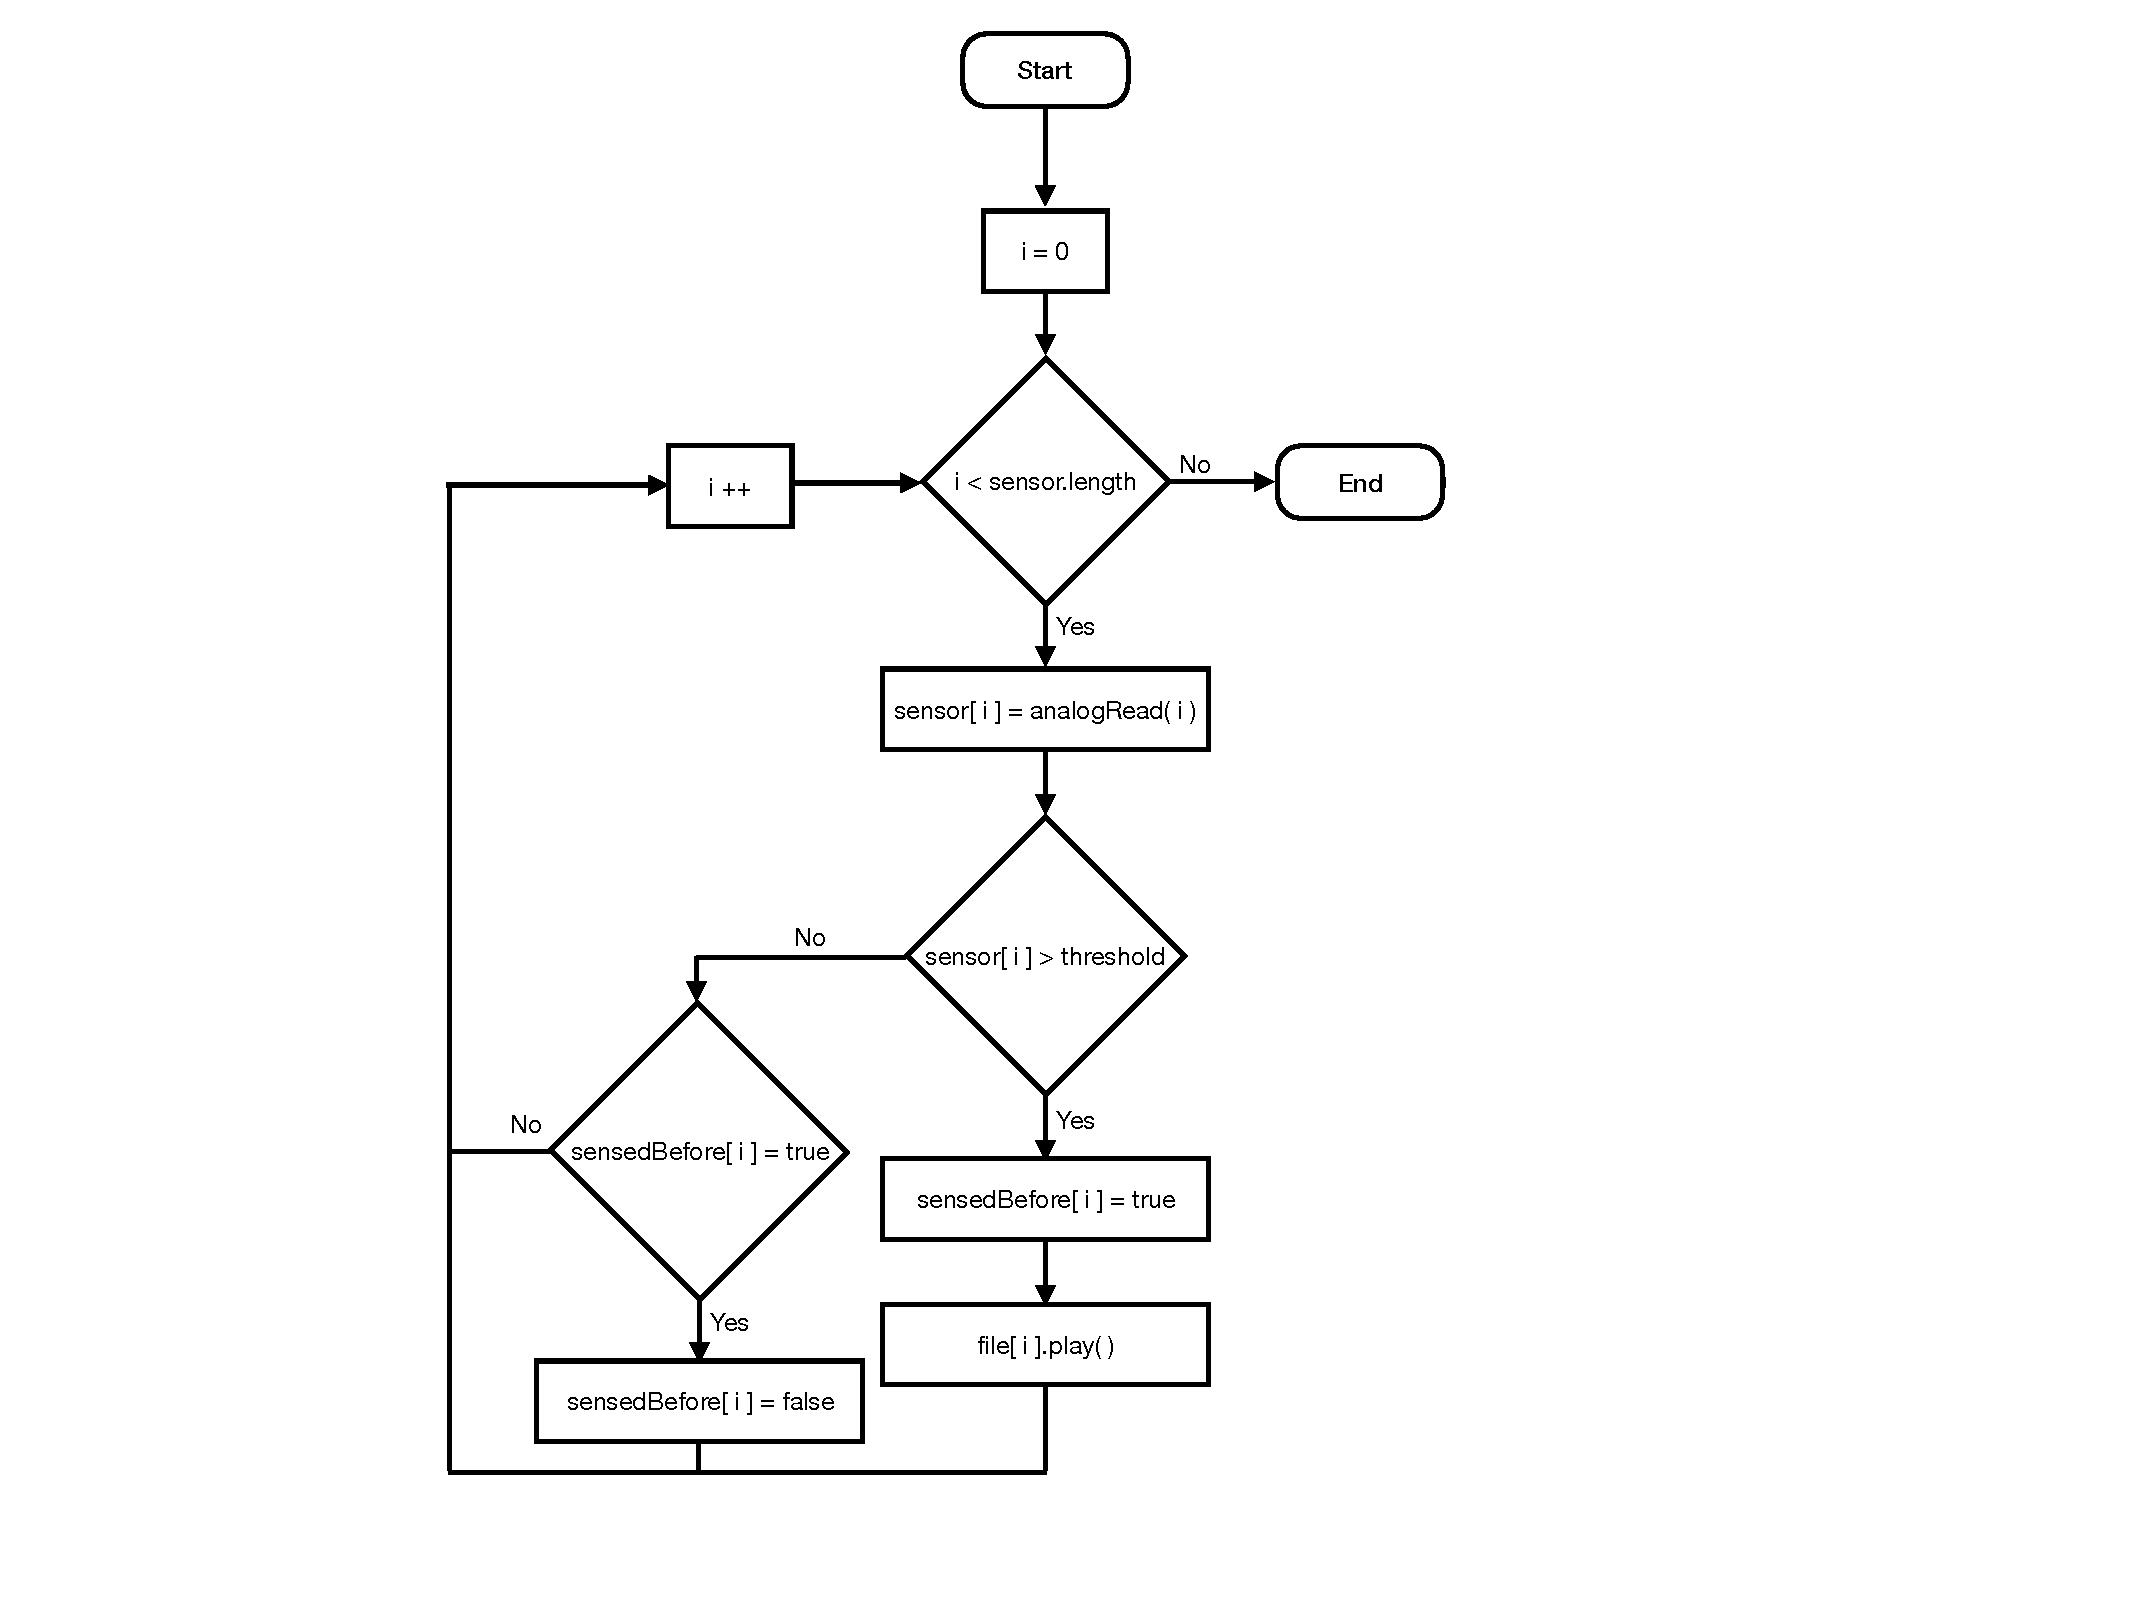
\includegraphics[scale=0.6]{Figure/protoFlowChart03.pdf}
\caption{
Flowchart for funktionen Afspil lyd. }
\label{fig:protoFlowChart03.pdf}
\end{figure}

 